%%%%%%%%%%%%%%%%%%%%%%%%%%%%%%%%%%%%%%%
%		NEWDatasetVIEW
%%%%%%%%%%%%%%%%%%%%%%%%%%%%%%%%%%%%%%%
\subsubsection{NewDatasetView (class)}
\label{speNdatV}
\begin{figure}[!h]
\centering
			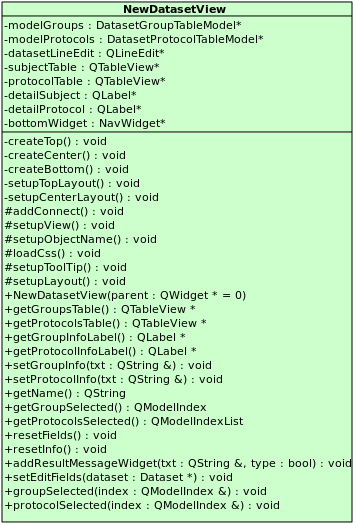
\includegraphics[width=0.5\linewidth]{./Content/Immagini/view/NewDatasetView.png}
			\caption{Classe NewDatasetView: attributi e metodi}
			\label{cl_ndatview}
\end{figure}
\paragraph{Descrizione \\}
Classe che rappresenta il widget per la creazione di un nuovo \dataset{}.
\paragraph{Utilizzo\\}
La classe implementerà i metodi virtuali puri della superclasse inoltre darà la possibilità all'utente di inserire un gruppo di \subject{} precedentemente creato, selezionare uno o più protocol\g{} da eseguire per quel gruppo di \subject{} e infine salvarlo.
\paragraph{Classi ereditate\\}
\begin{itemize}
\item Window::APanel.
\end{itemize}
%%%%%%%ATTRIBUTI%%%%%%%%%%%
\paragraph{\textcolor{black}{Attributi\\}}
\color{teal}\verb!-datasetLineEdit: QLineEdit*!
\begin{quote}
\color{black}Linea di testo che conterrà il nome del \dataset{} che l'utente sta andando a creare.
\end{quote}
%modelGroups
\color{teal}\verb!-modelGroups: DatasetGroupTableModel*!
\begin{quote}
\color{black}Modello che contiene 
\end{quote}
%modelProtocol
\color{teal}\verb!-modelProtocols: DatasetProtocolTableModel*!
\begin{quote}
\color{black}Modello che contiene tutti i \protocol{} che
\end{quote}
%detailSubject
\color{teal}\verb!-detailSubject: QLabel*!
\begin{quote}
\color{black}Contiene tutte le informazioni relative al \subject{} selezionato.
\end{quote}
%protocolTable
\color{teal}\verb!-ProtocolTable: QTableView*!
\begin{quote}
\color{black}Contiene la lista dei \protocol{} contenuti dentro a \emph{modelProtocols}
\end{quote}
%subjectTable
\color{teal}\verb!-detailProtocol: QTableView*!
\begin{quote}
\color{black}Contiene tutte le informazioni relative al \protocol{} selezionato.
\end{quote}
%bottomWidget
\color{teal}\verb! bottomWidget:NavWidget*!
\color{black} 
\begin{quote}
Puntatore al widget che rappresenta la parte bassa della finestra contentente i pulsanti necessari al salvataggio all'annullamento delle operazioni e tornare indietro.
\end{quote}
%%%%%%%%%%%% METODI %%%%%%%%%%%
\paragraph{\textcolor{black}{Metodi\\}}
%costruttore
\color{blue}\verb! + NewDatasetView(parent : QWidget*=0)!
\begin{quote}
\color{black}Costruttore per la classe NewDatasetView. \\
\textbf{Argomenti}
\begin{itemize}
\item parent: QWidget*=0  \\ Puntatore al QWidget padre di NewDatasetView.
\end{itemize}
\end{quote}
%setupLayout()
\color{blue}\verb! #setupLayout():void!
\begin{quote}
\color{black} Metodo che implementa il contratto fornito dalla classe astratta \hyperref[speAPanel]{APanel}.
\begin{itemize}
\item questo metodo deve essere marcato virtuale;
\item questo metodo è stato ridefinito.
\end{itemize}
\end{quote} 
%createTop
\color{blue}\verb! -createTop():void!
\begin{quote}
\color{black} Metodo che ha il compito di costruire la parte in alto del widget contenente la form per l'inserimento dei dati necessari per la creazione di un nuovo \dataset{}.
\end{quote} 
%createCenter
\color{blue}\verb! -createCenter():void!
\begin{quote}
\color{black} Metodo che ha il compito di costruire la parte centrale del widget per la vista che si occupa della  creazione di un nuovo \dataset{}.
\end{quote} 
%createButtom
\color{blue}\verb! -createButtom():void!
\begin{quote}
\color{black} Metodo che ha il compito di costruire la parte in basso del widget contenente il pulsante per ritornare alla pagine iniziale, il pulsante per il salvataggio e l'accesso alla guida.
\end{quote}
%setupTopLayout
\color{blue}\verb! -setupTopLayout():void!
\begin{quote}
\color{black} Metodo che ha il compito di impostare la parte alta del layout della finestra.
\end{quote}  
%setupCenterLayout()
\color{blue}\verb! -setupCenterLayout():void!
\begin{quote}
\color{black} Metodo che ha il compito di impostare la parte centrale del layout della finestra.
\end{quote} 
%LOADCSS
\color{blue}\verb! #loadCss():void!
\begin{quote}
\color{black} Metodo che implementa il contratto fornito dalla classe astratta \hyperref[speAPanel]{APanel}.\\
 \textbf{Note}
 \begin{itemize}
  \item questo metododeve essere marcato virtuale;
 \item questo metodo è stato ridefinito.
 \end{itemize}
\end{quote} 
%setupObjectName
\color{blue}\verb! #setupObjectName():void!
\begin{quote}
\color{black}Metodo che implementa il contratto fornito dalla classe astratta \hyperref[speAPanel]{APanel}.\\
 \textbf{Note}
 \begin{itemize}
  \item questo deve essere marcato virtuale;
 \item questo metodo è stato ridefinito.
 \end{itemize}
\end{quote} 
%setupToolTip
\color{blue}\verb! #setupToolTip():void!
\begin{quote}
\color{black}Metodo che implementa il contratto fornito dalla classe astratta \hyperref[speAPanel]{APanel}.\\
 \textbf{Note}
 \begin{itemize}
 \item questo metodo deve essere marcato virtuale;
 \item questo metodo è stato ridefinito.
 \end{itemize}
\end{quote} 
%addConnect
\color{blue}\verb! #addConnect():void!
\begin{quote}
\color{black}Metodo che implementa il contratto fornito dalla classe astratta \hyperref[speAPanel]{APanel}.\\
 \textbf{Note}
 \begin{itemize}
 \item questo metodo deve essere marcato costante;
 \item questo metodo deve essere marcato virtuale;
 \item questo metodo è stato ridefinito.
 \end{itemize}
\end{quote} 
%setupView
\color{blue}\verb! #setupView():void!
\begin{quote}
\color{black}Metodo che implementa il contratto fornito dalla classe astratta \hyperref[speAPanel]{APanel}.\\
 \textbf{Note}
 \begin{itemize}
 \item questo metodo deve essere marcato virtuale;
 \item questo metodo è stato ridefinito.
 \end{itemize}
\end{quote}
%getGroupTable
\color{blue}\verb! +getGroupTable(): QTableView*!
\begin{quote}
\color{black} Metodo che ritorna la lista dei gruppi di \subject{} disponibili.  \\
 \textbf{Note}
 \begin{itemize}
 \item questo metodo deve essere marcato costante.
 \end{itemize}
\end{quote}
%getProtocTable
\color{blue}\verb! +getProtocolsTable(): QTableView*!
\begin{quote}
\color{black} Metodo che ritorna la lista dei \protocol{} disponibili.\\
 \textbf{Note}
 \begin{itemize}
 \item questo metodo deve essere marcato costante.
 \end{itemize}
\end{quote} 
%getgroup
\color{blue}\verb! +getGroupInfoLabel(): QLabel*!
\begin{quote}
\color{black} Metodo che ritorna una label contenenente le informazioni relative al gruppo selezionato.  \\
 \textbf{Note}
 \begin{itemize}
 \item questo metodo deve essere marcato costante.
 \end{itemize}
\end{quote}
%getProto
\color{blue}\verb! +getProtocolInfoLabel(): QLabel*!
\begin{quote}
\color{black} Metodo che ritorna una label contenenente le informazioni relative al \protocol{} selezionato.  \\
 \textbf{Note}
 \begin{itemize}
 \item questo metodo deve essere marcato costante.
 \end{itemize}
\end{quote}
%setProtocolInfo
\color{blue}\verb! +setProtocolInfo(txt: QString&): void!
\begin{quote}
\color{black} Metodo che imposta le informazioni del protocol selezionato.  \\
 \textbf{Argomenti:}
 \begin{itemize}
 \item txt: QString\&\\ txt contiene il testo che verrà settato per il capo dati \emph{detailProtocol}.
 \end{itemize}
\end{quote}
%setGroupInfo
\color{blue}\verb! +setGroupInfo(txt: QString&): void!
\begin{quote}
\color{black} Metodo che imposta le informazioni del gruppo selezionato.  \\
 \textbf{Argomenti:}
 \begin{itemize}
 \item txt: QString\&\\ txt contiene il testo che verrà settato per il capo dati \emph{detailsSubject}.
 \end{itemize}
\end{quote}
%groupSelected
\color{blue}\verb! +groupSelected(index:QModelIndex&):void! (signal)
\color{black} 
\begin{quote}
Signal\g{} emesso quando l'utente seleziona un gruppo dalla tabella identificata dal campo dati \emph{subjectTable}.
\end{quote}
%protocolSelect
\color{blue}\verb! +groupSelected(index:QModelIndex&):void! (signal)
\color{black} 
\begin{quote}
Signal\g{} emesso quando l'utente seleziona un \protocol{} dalla tabella identificata dal campo dati \emph{protocolTable}.
\end{quote}
\pagebreak
\color{black}
%%%%%%%%%%%%%%%%%%%%%%%%%%%%%%%%%%
%		SUBJECTSVIEW
%%%%%%%%%%%%%%%%%%%%%%%%%%%%%%%%%%
\subsubsection{SubjectsView (class)}
\label{spesubV}
\begin{figure}[!h]
\centering
			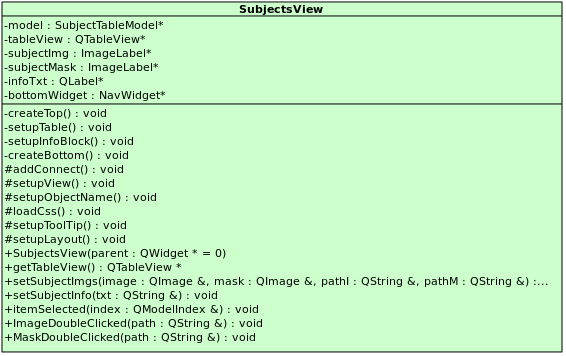
\includegraphics[width=0.5\linewidth]{./Content/Immagini/view/SubjectsView.png}
			\caption{Classe SubjectsView: attributi e metodi}
			\label{cl_subview}
\end{figure}
\paragraph{Descrizione \\}
Classe che rappresenta il widget per la visualizzazione di tutti i \subject{} presenti all'interno di \project.
\paragraph{Utilizzo\\}
La classe implementerà i metodi virtuali puri della superclasse inoltre darà la possibilità all'utente di visualizzare l'elenco di tutti i \subject{} fino a quel momento creati e memorizzati dentro a \project. Selezionando un \subject{} sarà possibile visualizzare le informazioni relative a quel \subject{}.
\paragraph{Classi ereditate\\}
\begin{itemize}
\item Window::APanel.
\end{itemize}
%%%%%%%ATTRIBUTI%%%%%%%%%%%
\paragraph{\textcolor{black}{Attributi\\}}
\color{teal}\verb!-model: SubjectTableModel *!
\begin{quote}
\color{black}Modello che contiene i \subject presenti nel sistema.
\end{quote}
%tabelView
\color{teal}\verb!-tableView: QTabelView*!
\color{black}
\begin{quote}
Contiene la lista dei \subject contenuti nel campo dati \emph{model}.
\end{quote}
%subjImg
\color{teal}\verb!-subjectImg: QLabel*!
\color{black}
\begin{quote}
Contiene l'immagine relativa al subject\g{} selezionato.
\end{quote}
%subjmask
\color{teal}\verb!-subjectMask: QLabel*!
\begin{quote}
\color{black}
Contiene la maschera relativa al subject\g{} selezionato.
\end{quote}
%infoTxt
\color{teal}\verb!-infoTxt: QLabel*!
\begin{quote}
\color{black}
Contiene le informazioni relative al \subject{} selezionato.
\end{quote}
%bottomWidget
\color{teal}\verb! bottomWidget:NavWidget*!
\color{black} 
\begin{quote}
Puntatore al widget che rappresenta la parte bassa della finestra contentente i pulsanti per tornare indietro e per la visualizzazione della guida interattiva.
\end{quote}
%%%%%%%%%  METODI
\paragraph{\textcolor{black}{Metodi\\}}
%costruttore
\color{blue}\verb! + SubjectsView(parent : QWidget*=0)!
\begin{quote}
\color{black}Costruttore per la classe SubjectsView. \\
\textbf{Argomenti}
\begin{itemize}
\item parent: QWidget*=0  \\ Puntatore al QWidget padre di SubjectsView.
\end{itemize}
\end{quote}
%setupLayout()
\color{blue}\verb! #setupLayout():void!
\begin{quote}
\color{black} Metodo che implementa il contratto fornito dalla classe astratta \hyperref[speAPanel]{APanel}.
\begin{itemize}
\item questo metodo deve essere marcato virtuale;
\item questo metodo è stato ridefinito.
\end{itemize}
\end{quote} 
%createTop
\color{blue}\verb! -createTop():void!
\begin{quote}
\color{black} Metodo che ha il compito di costruire la parte in alto del widget contenente l'elenco dei \subject e a lato lo spazio per visualizzare le informazioni.
\end{quote} 
%createButtom
\color{blue}\verb! -createButtom():void!
\begin{quote}
\color{black} Metodo che ha il compito di costruire la parte in basso del widget contenente il pulsante per ritornare alla pagine iniziale, e per l'accesso alla guida.
\end{quote}
%setupTable
%createButtom
\color{blue}\verb! -setupTable():void!
\begin{quote}
\color{black} Metodo che ha il compito di impostare la tabella che visualizzerà l'elenco dei \subject{} presenti nel sistema.
\end{quote}
%createButtom
\color{blue}\verb! -setupInfoBlock():void!
\begin{quote}
\color{black} Metodo che ha il compito di impostare il layout riguardante la visualizzazione delle informazioni.
\end{quote}
%LOADCSS
\color{blue}\verb! #loadCss():void!
\begin{quote}
\color{black} Metodo che implementa il contratto fornito dalla classe astratta \hyperref[speAPanel]{APanel}.\\
 \textbf{Note}
 \begin{itemize}
  \item questo metododeve essere marcato virtuale;
 \item questo metodo è stato ridefinito.
 \end{itemize}
\end{quote} 
%setupObjectName
\color{blue}\verb! #setupObjectName():void!
\begin{quote}
\color{black}Metodo che implementa il contratto fornito dalla classe astratta \hyperref[speAPanel]{APanel}.\\
 \textbf{Note}
 \begin{itemize}
  \item questo deve essere marcato virtuale;
 \item questo metodo è stato ridefinito.
 \end{itemize}
\end{quote} 
%setupToolTip
\color{blue}\verb! #setupToolTip():void!
\begin{quote}
\color{black}Metodo che implementa il contratto fornito dalla classe astratta \hyperref[speAPanel]{APanel}.\\
 \textbf{Note}
 \begin{itemize}
 \item questo metodo deve essere marcato virtuale;
 \item questo metodo è stato ridefinito.
 \end{itemize}
\end{quote} 
%addConnect
\color{blue}\verb! #addConnect():void!
\begin{quote}
\color{black}Metodo che implementa il contratto fornito dalla classe astratta \hyperref[speAPanel]{APanel}.\\
 \textbf{Note}
 \begin{itemize}
 \item questo metodo deve essere marcato costante;
 \item questo metodo deve essere marcato virtuale;
 \item questo metodo è stato ridefinito.
 \end{itemize}
\end{quote} 
%setupView
\color{blue}\verb! #setupView():void!
\begin{quote}
\color{black}Metodo che implementa il contratto fornito dalla classe astratta \hyperref[speAPanel]{APanel}.\\
 \textbf{Note}
 \begin{itemize}
 \item questo metodo deve essere marcato virtuale;
 \item questo metodo è stato ridefinito.
 \end{itemize}
\end{quote}
%subjView
\color{blue}\verb! -getTableView():QTabelView*!
\begin{quote}
\color{black}Metodo che ritorna il puntatore campo dati \emph{tableView}.\\
 \textbf{Note}
 \begin{itemize}
 \item questo metodo deve essere marcato costante.
 \end{itemize}
\end{quote}
%setsubjImg
\color{blue}\verb! -setSubjectImg(imgage:QImage&):void!
\begin{quote}
\color{black}Metodo che imposta l'immagine del \subject{} nella parte delle informazioni relative al \subject{}.\\
\textbf{Argomenti:}
\begin{itemize}
\item image: QImage\& \\ contiene l'immagine che verrà impostata nella parte delle informazioni.
\end{itemize}
\end{quote}
%setsubjmask
\color{blue}\verb! -setSubjectMask(imgage:QImage&):void!
\begin{quote}
\color{black}Metodo che imposta la maschera del \subject{} nella parte delle informazioni relative al \subject{}.\\
\textbf{Argomenti:}
\begin{itemize}
\item image: QImage\& \\ contiene la maschera che verrà impostata nella parte delle informazioni.
\end{itemize}
\end{quote}
%setSubjectInfo
\color{blue}\verb! -setSubjectInfo(txt:QString&):void!
\begin{quote}
\color{black}Metodo che imposta tutte le informazioni del \subject selezionato nella parte deidicata alle informazioni.\\
\textbf{Argomenti:}
\begin{itemize}
\item txt: QString\& \\ stringa contenente le nuove informazioni da visualizzare.
\end{itemize}
\end{quote}
%itemSelected
\color{blue}\verb! +itemSelected(index:QModelIndex&):void! (signal)
\color{black} 
\begin{quote}
Signal\g{} emesso quando l'utente seleziona un \subject{} dalla tabella contenente tutti i \subject{} presenti.
\end{quote}
\pagebreak
\color{black}
%%%%%%%%%%%%%%
%	GROUPVIEW
%%%%%%%%%%%%%%%%
\subsubsection{GroupView (class)}
\label{spegroV}
\begin{figure}[!h]
\centering
			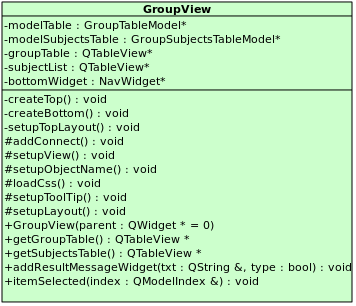
\includegraphics[width=0.5\linewidth]{./Content/Immagini/view/GroupView.png}
			\caption{Classe GroupView: attributi e metodi}
			\label{cl_groview}
\end{figure}
\paragraph{Descrizione \\}
Classe che rappresenta il widget per la visualizzazione di tutti i gruppi di \subject{} presenti all'interno di \project.
\paragraph{Utilizzo\\}
La classe implementerà i metodi virtuali puri della superclasse inoltre darà la possibilità all'utente di visualizzare l'elenco di tutti i gruppi di \subject{} fino a quel momento creati e memorizzati dentro a \project. Selezionando un gruppo, sarà possibile visualizzare le informazioni relative a quel gruppo, come per esempio i \subject{} contenuti al suo interno.
\paragraph{Classi ereditate\\}
\begin{itemize}
\item Window::APanel.
\end{itemize}
%%%%%%%ATTRIBUTI%%%%%%%%%%%
\paragraph{\textcolor{black}{Attributi\\}}
\color{teal}\verb!-modelTable: GroupTableModel *!
\begin{quote}
\color{black}Modello che contiene i gruppi di\subject{} presenti nel sistema fino a quel momento.
\end{quote}
%modelSub
\color{teal}\verb!-modeSubjectslTable: GroupSubjectsTableModel *!
\begin{quote}
\color{black}Modello che contiene i \subject{} presenti in un determinato gruppo di \subject{} fino a quel momento presenti nel sistema.
\end{quote}
%tabelView
\color{teal}\verb!-groupTable: QTabelView*!
\color{black}
\begin{quote}
Contiene la lista dei gruppi di \subject{} contenuti nel campo dati \emph{modelTable}.
\end{quote}
%tabelView
\color{teal}\verb!-subjectList: QTabelView*!
\color{black}
\begin{quote}
Contiene la lista dei \subject{} contenuti nel campo dati \emph{modelSubjectsTable}.
\end{quote}
%bottomWidget
\color{teal}\verb! bottomWidget:NavWidget*!
\color{black} 
\begin{quote}
Puntatore al widget che rappresenta la parte bassa della finestra contentente i pulsanti per tornare indietro, la visualizzazione della guida interattiva, la possibilità di editare un gruppo e salvare successivamente le modifiche.
\end{quote}
%%%%%%%%%  METODI
\paragraph{\textcolor{black}{Metodi\\}}
%costruttore
\color{blue}\verb! + GroupView(parent : QWidget*=0)!
\begin{quote}
\color{black}Costruttore per la classe GroupView. \\
\textbf{Argomenti}
\begin{itemize}
\item parent: QWidget*=0  \\ Puntatore al QWidget padre di GroupView.
\end{itemize}
\end{quote}
%setupLayout()
\color{blue}\verb! #setupLayout():void!
\begin{quote}
\color{black} Metodo che implementa il contratto fornito dalla classe astratta \hyperref[speAPanel]{APanel}.
\begin{itemize}
\item questo metodo deve essere marcato virtuale;
\item questo metodo è stato ridefinito.
\end{itemize}
\end{quote} 
%createTop
\color{blue}\verb! -createTop():void!
\begin{quote}
\color{black} Metodo che ha il compito di costruire la parte in alto del widget contenente l'elenco dei \subject e a lato lo spazio per visualizzare le informazioni.
\end{quote} 
%createButtom
\color{blue}\verb! -createButtom():void!
\begin{quote}
\color{black} Metodo che ha il compito di costruire la parte in basso del widget contenente il pulsante per ritornare alla pagine iniziale, e per l'accesso alla guida.
\end{quote}
%setupTopLayout
\color{blue}\verb! -setupTopLayout():void!
\begin{quote}
\color{black} Metodo che ha il compito di impostare la parte alta del layout della finestra.
\end{quote}  
%LOADCSS
\color{blue}\verb! #loadCss():void!
\begin{quote}
\color{black} Metodo che implementa il contratto fornito dalla classe astratta \hyperref[speAPanel]{APanel}.\\
 \textbf{Note}
 \begin{itemize}
  \item questo metododeve essere marcato virtuale;
 \item questo metodo è stato ridefinito.
 \end{itemize}
\end{quote} 
%setupObjectName
\color{blue}\verb! #setupObjectName():void!
\begin{quote}
\color{black}Metodo che implementa il contratto fornito dalla classe astratta \hyperref[speAPanel]{APanel}.\\
 \textbf{Note}
 \begin{itemize}
  \item questo deve essere marcato virtuale;
 \item questo metodo è stato ridefinito.
 \end{itemize}
\end{quote} 
%setupToolTip
\color{blue}\verb! #setupToolTip():void!
\begin{quote}
\color{black}Metodo che implementa il contratto fornito dalla classe astratta \hyperref[speAPanel]{APanel}.\\
 \textbf{Note}
 \begin{itemize}
 \item questo metodo deve essere marcato virtuale;
 \item questo metodo è stato ridefinito.
 \end{itemize}
\end{quote} 
%addConnect
\color{blue}\verb! #addConnect():void!
\begin{quote}
\color{black}Metodo che implementa il contratto fornito dalla classe astratta \hyperref[speAPanel]{APanel}.\\
 \textbf{Note}
 \begin{itemize}
 \item questo metodo deve essere marcato costante;
 \item questo metodo deve essere marcato virtuale;
 \item questo metodo è stato ridefinito.
 \end{itemize}
\end{quote} 
%setupView
\color{blue}\verb! #setupView():void!
\begin{quote}
\color{black}Metodo che implementa il contratto fornito dalla classe astratta \hyperref[speAPanel]{APanel}.\\
 \textbf{Note}
 \begin{itemize}
 \item questo metodo deve essere marcato virtuale;
 \item questo metodo è stato ridefinito.
 \end{itemize}
\end{quote}
%getGroup
\color{blue}\verb! -getGroup():QTabelView*!
\begin{quote}
\color{black}Metodo che ritorna il puntatore al campo dati \emph{groupTable}.\\
 \textbf{Note}
 \begin{itemize}
 \item questo metodo deve essere marcato costante.
 \end{itemize}
\end{quote}
%getsubje
\color{blue}\verb! -getSubjectsTable():QTabelView*!
\begin{quote}
\color{black}Metodo che ritorna il puntatore al campo dati \emph{modelSubjectTable}.\\
 \textbf{Note}
 \begin{itemize}
 \item questo metodo deve essere marcato costante.
 \end{itemize}
\end{quote}
%itemSelected
\color{blue}\verb! +itemSelected(index:QModelIndex&)! (signal)
\color{black} 
\begin{quote}
Signal\g{} emesso quando l'utente seleziona un elemento da una tabella, che sia quella contentente la lista di gruppi di \subject{} o quella con la lista dei \subject{} per un determinato gruppo.
\end{quote}
\pagebreak
\color{black}
%%%%%%%%%%%%%%%%%%%%%%
% PROTOCOLSVIEW
%%%%%%%%%%%%%%%%%%%%%
\subsubsection{ProtocolsView (class)}
\label{speproV}
\begin{figure}[!h]
\centering
			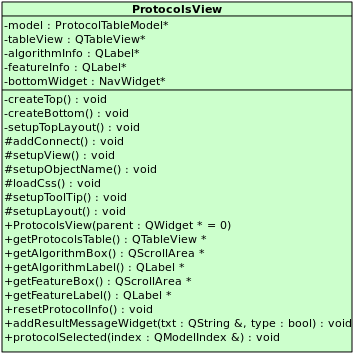
\includegraphics[width=0.5\linewidth]{./Content/Immagini/view/ProtocolsView.png}
			\caption{Classe ProtocolsView: attributi e metodi}
			\label{cl_proview}
\end{figure}
\paragraph{Descrizione \\}
Classe che rappresenta il widget per la visualizzazione di tutti i \protocol{} presenti all'interno di \project.
\paragraph{Utilizzo\\}
La classe implementerà i metodi virtuali puri della superclasse inoltre darà la possibilità all'utente di visualizzare l'elenco di tutti i \protocol{} fino a quel momento creati e memorizzati dentro a \project. Selezionando un \protocol{}, sarà possibile visualizzare le informazioni relative a quel \protocol{}: feature\g{} presenti con il valore dei parametri (qualora fossero presenti), e algoritmo di clustering\g{} con valore dei parametri.
\paragraph{Classi ereditate\\}
\begin{itemize}
\item Window::APanel.
\end{itemize}
%%%%%%%ATTRIBUTI%%%%%%%%%%%
\paragraph{\textcolor{black}{Attributi\\}}
\color{teal}\verb!-model: protocolTableModel *!
\begin{quote}
\color{black}Modello che contiene i \protocol{} presenti nel sistema fino a quel momento.
\end{quote}
%tabelView
\color{teal}\verb!-tableView: QTabelView*!
\color{black}
\begin{quote}
Contiene la lista dei \protocol{} contenuti nel campo dati \emph{model}.
\end{quote}
%algInfo
\color{teal}\verb!-algorithmInfo: QLabel*!
\begin{quote}
\color{black}
Contiene le informazioni relative all'algoritmo di clustering\g{} del \protocol{} selezionato, qualora fosse presente.
\end{quote}
%featInfo
\color{teal}\verb!-featureInfo: QLabel*!
\color{black}
\begin{quote}
Contiene le informazioni relative alle Feature\g{} del \protocol{} selezionato qualora fosse presente almeno una Feature\g{}.
\end{quote}
%bottomWidget
\color{teal}\verb! bottomWidget:NavWidget*!
\color{black} 
\begin{quote}
Puntatore al widget che rappresenta la parte bassa della finestra contentente i pulsanti per tornare indietro, la visualizzazione della guida interattiva, la possibilità di eliminare un \protocol{} e confermare l'operazione.
\end{quote}
%%%%%%%%%  METODI
\paragraph{\textcolor{black}{Metodi\\}}
%costruttore
\color{blue}\verb! + ProtocolsView(parent : QWidget*=0)!
\begin{quote}
\color{black}Costruttore per la classe ProtocolsView. \\
\textbf{Argomenti}
\begin{itemize}
\item parent: QWidget*=0  \\ Puntatore al QWidget padre di ProtocolsView.
\end{itemize}
\end{quote}
%setupLayout()
\color{blue}\verb! #setupLayout():void!
\begin{quote}
\color{black} Metodo che implementa il contratto fornito dalla classe astratta \hyperref[speAPanel]{APanel}.
\begin{itemize}
\item questo metodo deve essere marcato virtuale;
\item questo metodo è stato ridefinito.
\end{itemize}
\end{quote} 
%createTop
\color{blue}\verb! -createTop():void!
\begin{quote}
\color{black} Metodo che ha il compito di costruire la parte in alto del widget contenente l'elenco dei \subject e a lato lo spazio per visualizzare le informazioni.
\end{quote} 
%createButtom
\color{blue}\verb! -createButtom():void!
\begin{quote}
\color{black} Metodo che ha il compito di costruire la parte in basso del widget contenente il pulsante per ritornare alla pagine iniziale, e per l'accesso alla guida.
\end{quote}
%setupTopLayout
\color{blue}\verb! -setupTopLayout():void!
\begin{quote}
\color{black} Metodo che ha il compito di impostare la parte alta del layout della finestra.
\end{quote}  
%LOADCSS
\color{blue}\verb! #loadCss():void!
\begin{quote}
\color{black} Metodo che implementa il contratto fornito dalla classe astratta \hyperref[speAPanel]{APanel}.\\
 \textbf{Note}
 \begin{itemize}
  \item questo metododeve essere marcato virtuale;
 \item questo metodo è stato ridefinito.
 \end{itemize}
\end{quote} 
%setupObjectName
\color{blue}\verb! #setupObjectName():void!
\begin{quote}
\color{black}Metodo che implementa il contratto fornito dalla classe astratta \hyperref[speAPanel]{APanel}.\\
 \textbf{Note}
 \begin{itemize}
  \item questo deve essere marcato virtuale;
 \item questo metodo è stato ridefinito.
 \end{itemize}
\end{quote} 
%setupToolTip
\color{blue}\verb! #setupToolTip():void!
\begin{quote}
\color{black}Metodo che implementa il contratto fornito dalla classe astratta \hyperref[speAPanel]{APanel}.\\
 \textbf{Note}
 \begin{itemize}
 \item questo metodo deve essere marcato virtuale;
 \item questo metodo è stato ridefinito.
 \end{itemize}
\end{quote} 
%addConnect
\color{blue}\verb! #addConnect():void!
\begin{quote}
\color{black}Metodo che implementa il contratto fornito dalla classe astratta \hyperref[speAPanel]{APanel}.\\
 \textbf{Note}
 \begin{itemize}
 \item questo metodo deve essere marcato costante;
 \item questo metodo deve essere marcato virtuale;
 \item questo metodo è stato ridefinito.
 \end{itemize}
\end{quote} 
%setupView
\color{blue}\verb! #setupView():void!
\begin{quote}
\color{black}Metodo che implementa il contratto fornito dalla classe astratta \hyperref[speAPanel]{APanel}.\\
 \textbf{Note}
 \begin{itemize}
 \item questo metodo deve essere marcato virtuale;
 \item questo metodo è stato ridefinito.
 \end{itemize}
\end{quote}
%getAlgInfo
\color{blue}\verb! -getAlgorithmLabel():QLabel*!
\begin{quote}
\color{black}Metodo che ritorna la label contenente le informazioni riguardanti l'algoritmo di clustering\g{} presente nel \protocol{}.\\
 \textbf{Note}
 \begin{itemize}
 \item questo metodo deve essere marcato costante.
 \end{itemize}
\end{quote}
%getInf
\color{blue}\verb! -getFeatureLabel():QLabel*!
\begin{quote}
\color{black}Metodo che ritorna la label contenente le informazioni riguardanti le Feature\g{} presenti nel \protocol{}.\\
 \textbf{Note}
 \begin{itemize}
 \item questo metodo deve essere marcato costante.
 \end{itemize}
\end{quote}
%protSelected
\color{blue}\verb! +protocolSelected(index:QModelIndex&):void! (signal)
\color{black} 
\begin{quote}
Signal\g{} emesso quando l'utente seleziona un elemento da una tabella, che sia quella contentente la lista di gruppi di \subject{} o quella con la lista dei \subject{} per un determinato gruppo.
\end{quote}
%%%%%%%%%%%%%%%%%%%%5
%	DATASETSVIEW
%%%%%%%%%%%%%%%%
\subsubsection{DatasetsView (class)}
\label{spedatV}
\begin{figure}[!h]
\centering
			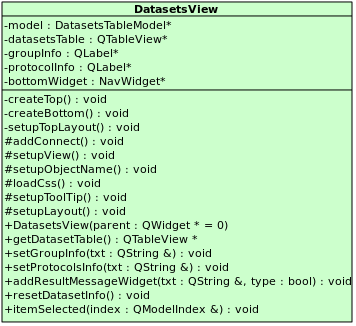
\includegraphics[width=0.5\linewidth]{./Content/Immagini/view/DatasetsView.png}
			\caption{Classe DatasetsView: attributi e metodi}
			\label{cl_datview}
\end{figure}
\paragraph{Descrizione \\}
Classe che rappresenta il widget per la visualizzazione di tutti i \dataset{} presenti all'interno di \project.
\paragraph{Utilizzo\\}
La classe implementerà i metodi virtuali puri della superclasse inoltre darà la possibilità all'utente di visualizzare l'elenco di tutti i \dataset{} fino a quel momento creati e memorizzati dentro a \project. Selezionando un \dataset{}, sarà possibile visualizzare le informazioni relative a quel \dataset{}: gruppo di \subject{} contenuto e \protocol{} presenti (uno o più).
\paragraph{Classi ereditate\\}
\begin{itemize}
\item Window::APanel.
\end{itemize}
%%%%%%%ATTRIBUTI%%%%%%%%%%%
\paragraph{\textcolor{black}{Attributi\\}}

%tabelView
\color{teal}\verb!-DatasetsView: QTabelView*!
\color{black}
\begin{quote}
Contiene la lista dei \dataset{} contenuti nel campo dati 
\end{quote}
%algInfo
\color{teal}\verb!-algorithmInfo: QLabel*!
\color{black}
\begin{quote}
Contiene le informazioni relative all'algoritmo di clustering\g{} del \protocol{} selezionato, qualora fosse presente.
\end{quote}
%featInfo
\color{teal}\verb!-featureInfo: QLabel*!
\color{black}
\begin{quote}
Contiene le informazioni relative alle Feature\g{} del \protocol{} selezionato qualora fosse presente almeno una Feature\g{}.
\end{quote}
%bottomWidget
\color{teal}\verb! bottomWidget:NavWidget*!
\color{black} 
\begin{quote}
Puntatore al widget che rappresenta la parte bassa della finestra contentente i pulsanti per tornare indietro, la visualizzazione della guida interattiva, la possibilità di eliminare un \dataset{} e confermare successivamente l'operazione.
\end{quote}
%%%%%%%%%  METODI
\paragraph{\textcolor{black}{Metodi\\}}
%costruttore
\color{blue}\verb! + DatasetsView(parent : QWidget*=0)!
\begin{quote}
\color{black}Costruttore per la classe DatasesView. \\
\textbf{Argomenti}
\begin{itemize}
\item parent: QWidget*=0  \\ Puntatore al QWidget padre di DatasetsView.
\end{itemize}
\end{quote}
%setupLayout()
\color{blue}\verb! #setupLayout():void!
\begin{quote}
\color{black} Metodo che implementa il contratto fornito dalla classe astratta \hyperref[speAPanel]{APanel}.
\begin{itemize}
\item questo metodo deve essere marcato virtuale;
\item questo metodo è stato ridefinito.
\end{itemize}
\end{quote} 
%createTop
\color{blue}\verb! -createTop():void!
\begin{quote}
\color{black} Metodo che ha il compito di costruire la parte in alto del widget contenente l'elenco dei \subject e a lato lo spazio per visualizzare le informazioni.
\end{quote} 
%createButtom
\color{blue}\verb! -createButtom():void!
\begin{quote}
\color{black} Metodo che ha il compito di costruire la parte in basso del widget contenente il pulsante per ritornare alla pagine iniziale, e per l'accesso alla guida.
\end{quote}
%setupTopLayout
\color{blue}\verb! -setupTopLayout():void!
\begin{quote}
\color{black} Metodo che ha il compito di impostare la parte alta del layout della finestra.
\end{quote}  
%LOADCSS
\color{blue}\verb! #loadCss():void!
\begin{quote}
\color{black} Metodo che implementa il contratto fornito dalla classe astratta \hyperref[speAPanel]{APanel}.\\
 \textbf{Note}
 \begin{itemize}
  \item questo metododeve essere marcato virtuale;
 \item questo metodo è stato ridefinito.
 \end{itemize}
\end{quote} 
%setupObjectName
\color{blue}\verb! #setupObjectName():void!
\begin{quote}
\color{black}Metodo che implementa il contratto fornito dalla classe astratta \hyperref[speAPanel]{APanel}.\\
 \textbf{Note}
 \begin{itemize}
  \item questo deve essere marcato virtuale;
 \item questo metodo è stato ridefinito.
 \end{itemize}
\end{quote} 
%setupToolTip
\color{blue}\verb! #setupToolTip():void!
\begin{quote}
\color{black}Metodo che implementa il contratto fornito dalla classe astratta \hyperref[speAPanel]{APanel}.\\
 \textbf{Note}
 \begin{itemize}
 \item questo metodo deve essere marcato virtuale;
 \item questo metodo è stato ridefinito.
 \end{itemize}
\end{quote} 
%addConnect
\color{blue}\verb! #addConnect():void!
\begin{quote}
\color{black}Metodo che implementa il contratto fornito dalla classe astratta \hyperref[speAPanel]{APanel}.\\
 \textbf{Note}
 \begin{itemize}
 \item questo metodo deve essere marcato costante;
 \item questo metodo deve essere marcato virtuale;
 \item questo metodo è stato ridefinito.
 \end{itemize}
\end{quote} 
%setupView
\color{blue}\verb! #setupView():void!
\begin{quote}
\color{black}Metodo che implementa il contratto fornito dalla classe astratta \hyperref[speAPanel]{APanel}.\\
 \textbf{Note}
 \begin{itemize}
 \item questo metodo deve essere marcato virtuale;
 \item questo metodo è stato ridefinito.
 \end{itemize}
\end{quote}
\pagebreak
\color{black}
%%%%%%%%%%%%%%%%%%%%
% 		ANALYSIS
%%%%%%%%%%%%%%%%%
\subsubsection{AnalysisView (class)}
\label{speanaV}
\begin{figure}[!h]
\centering
			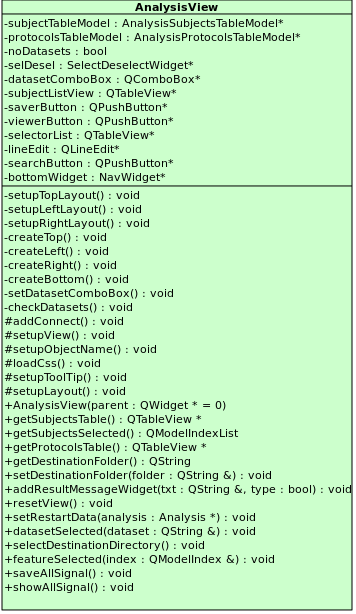
\includegraphics[width=0.5\linewidth]{./Content/Immagini/view/AnalysisView.png}
			\caption{Classe AnalysisView: attributi e metodi}
			\label{cl_anaview}
\end{figure}
\paragraph{Descrizione \\}
Classe che rappresenta il widget per avviare un'analisi su un \dataset{}.
\paragraph{Utilizzo\\}
La classe implementerà i metodi virtuali puri della superclasse inoltre darà la possibilità all'utente di selezionare un \dataset{} sul quale effettuare un'analisi,selezionare quali \subject{} analizzare, scegliere quali risultati salvare per le Feature\g{} (per l'algoritmo, di default viene sia visualizzato, sia esportato), selezionare il path di dove salvare i risultati e infine far partire l'analisi.
\paragraph{Classi ereditate\\}
\begin{itemize}
\item Window::APanel.
\end{itemize}
%%%%%%%ATTRIBUTI%%%%%%%%%%%
\paragraph{\textcolor{black}{Attributi\\}}

%tabelView
\color{teal}\verb!-DatasetsView: QTabelView*!
\color{black}
\begin{quote}
Contiene la lista dei \dataset{} contenuti nel campo dati 
\end{quote}
%algInfo
\color{teal}\verb!-algorithmInfo: QLabel*!
\color{black}
\begin{quote}
Contiene le informazioni relative all'algoritmo di clustering\g{} del \protocol{} selezionato, qualora fosse presente.
\end{quote}
%featInfo
\color{teal}\verb!-featureInfo: QLabel*!
\color{black}
\begin{quote}
Contiene le informazioni relative alle Feature\g{} del \protocol{} selezionato qualora fosse presente almeno una Feature\g{}.
\end{quote}
%bottomWidget
\color{teal}\verb! bottomWidget:NavWidget*!
\color{black} 
\begin{quote}
Puntatore al widget che rappresenta la parte bassa della finestra contentente i pulsanti per tornare indietro, la visualizzazione della guida interattiva, la possibilità di eliminare un \dataset{} e confermare successivamente l'operazione.
\end{quote}
%%%%%%%%%  METODI
\paragraph{\textcolor{black}{Metodi\\}}
%costruttore
\color{blue}\verb! + DatasetsView(parent : QWidget*=0)!
\begin{quote}
\color{black}Costruttore per la classe DatasesView. \\
\textbf{Argomenti}
\begin{itemize}
\item parent: QWidget*=0  \\ Puntatore al QWidget padre di DatasetsView.
\end{itemize}
\end{quote}
%setupLayout()
\color{blue}\verb! #setupLayout():void!
\begin{quote}
\color{black} Metodo che implementa il contratto fornito dalla classe astratta \hyperref[speAPanel]{APanel}.
\begin{itemize}
\item questo metodo deve essere marcato virtuale;
\item questo metodo è stato ridefinito.
\end{itemize}
\end{quote} 
%createTop
\color{blue}\verb! -createTop():void!
\begin{quote}
\color{black} Metodo che ha il compito di costruire la parte in alto del widget contenente l'elenco dei \subject e a lato lo spazio per visualizzare le informazioni.
\end{quote} 
%createButtom
\color{blue}\verb! -createButtom():void!
\begin{quote}
\color{black} Metodo che ha il compito di costruire la parte in basso del widget contenente il pulsante per ritornare alla pagine iniziale, e per l'accesso alla guida.
\end{quote}
%setupTopLayout
\color{blue}\verb! -setupTopLayout():void!
\begin{quote}
\color{black} Metodo che ha il compito di impostare la parte alta del layout della finestra.
\end{quote}  
%LOADCSS
\color{blue}\verb! #loadCss():void!
\begin{quote}
\color{black} Metodo che implementa il contratto fornito dalla classe astratta \hyperref[speAPanel]{APanel}.\\
 \textbf{Note}
 \begin{itemize}
  \item questo metododeve essere marcato virtuale;
 \item questo metodo è stato ridefinito.
 \end{itemize}
\end{quote} 
%setupObjectName
\color{blue}\verb! #setupObjectName():void!
\begin{quote}
\color{black}Metodo che implementa il contratto fornito dalla classe astratta \hyperref[speAPanel]{APanel}.\\
 \textbf{Note}
 \begin{itemize}
  \item questo deve essere marcato virtuale;
 \item questo metodo è stato ridefinito.
 \end{itemize}
\end{quote} 
%setupToolTip
\color{blue}\verb! #setupToolTip():void!
\begin{quote}
\color{black}Metodo che implementa il contratto fornito dalla classe astratta \hyperref[speAPanel]{APanel}.\\
 \textbf{Note}
 \begin{itemize}
 \item questo metodo deve essere marcato virtuale;
 \item questo metodo è stato ridefinito.
 \end{itemize}
\end{quote} 
%addConnect
\color{blue}\verb! #addConnect():void!
\begin{quote}
\color{black}Metodo che implementa il contratto fornito dalla classe astratta \hyperref[speAPanel]{APanel}.\\
 \textbf{Note}
 \begin{itemize}
 \item questo metodo deve essere marcato costante;
 \item questo metodo deve essere marcato virtuale;
 \item questo metodo è stato ridefinito.
 \end{itemize}
\end{quote} 
%setupView
\color{blue}\verb! #setupView():void!
\begin{quote}
\color{black}Metodo che implementa il contratto fornito dalla classe astratta \hyperref[speAPanel]{APanel}.\\
 \textbf{Note}
 \begin{itemize}
 \item questo metodo deve essere marcato virtuale;
 \item questo metodo è stato ridefinito.
 \end{itemize}
\end{quote}
\pagebreak
\color{black}
%%%%%%%%%%%%%%%%%%%%%%%%
%	DETAILED	
%%%%%%%%%%%%%%%%%
\subsubsection{DetailedResult (class)}
\label{spedetRe}
\begin{figure}[!h]
\centering
			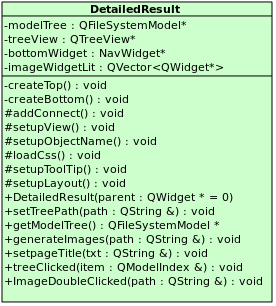
\includegraphics[width=0.5\linewidth]{./Content/Immagini/view/DetailedResult.png}
			\caption{Classe DetailedResult: attributi e metodi}
			\label{cl_detRes}
\end{figure}
\paragraph{Descrizione \\}
Classe che rappresenta il widget per la visualizzazione di tutti i gruppi di \subject{} presenti all'interno di \project.
\paragraph{Utilizzo\\}
La classe implementerà i metodi virtuali puri della superclasse inoltre darà la possibilità all'utente di visualizzare l'elenco di tutti i gruppi di \subject{} fino a quel momento creati e memorizzati dentro a \project. Selezionando un gruppo, sarà possibile visualizzare le informazioni relative a quel gruppo, come per esempio i \subject{} contenuti al suo interno.
\paragraph{Classi ereditate\\}
\begin{itemize}
\item Window::APanel.
\end{itemize}
%%%%%%%ATTRIBUTI%%%%%%%%%%%
\paragraph{\textcolor{black}{Attributi\\}}
%treeView
\color{teal}\verb!-treeView: QTreeView*!
\color{black}
\begin{quote}
Rappresenta l'albero dei risultati di un'analisi. L'albero è ordinabile per l'elenco dei \subject{} su cui è stata effettuata l'analisi oppure per \protocol{} presenti nel \dataset{} su cui è stata eseguita l'analisi.
\end{quote}
%tabelView
\color{teal}\verb!-ListView: QListView*!
\color{black}
\begin{quote}
Contiene la lista di risultati che l'utente ha scelto di visualizzare, cliccando da \emph{treeView} una voce dell'albero.
\end{quote}
%bottomWidget
\color{teal}\verb! bottomWidget:NavWidget*!
\color{black} 
\begin{quote}
Puntatore al widget che rappresenta la parte bassa della finestra contentente i pulsanti per tornare indietro,e la visualizzazione della guida interattiva.
\end{quote}
%%%%%%%%%  METODI
\paragraph{\textcolor{black}{Metodi\\}}
%costruttore
\color{blue}\verb! + DetailedResult(parent : QWidget*=0)!
\begin{quote}
\color{black}Costruttore per la classe DetailedResult. \\
\textbf{Argomenti}
\begin{itemize}
\item parent: QWidget*=0  \\ Puntatore al QWidget padre di DetailedResult.
\end{itemize}
\end{quote}
%setupLayout()
\color{blue}\verb! #setupLayout():void!
\begin{quote}
\color{black} Metodo che implementa il contratto fornito dalla classe astratta \hyperref[speAPanel]{APanel}.
\begin{itemize}
\item questo metodo deve essere marcato virtuale;
\item questo metodo è stato ridefinito.
\end{itemize}
\end{quote} 
%createTop
\color{blue}\verb! -createTop():void!
\begin{quote}
\color{black} Metodo che ha il compito di costruire la parte in alto del widget contenente l'elenco dei \subject e a lato lo spazio per visualizzare le informazioni.
\end{quote} 
%createButtom
\color{blue}\verb! -createButtom():void!
\begin{quote}
\color{black} Metodo che ha il compito di costruire la parte in basso del widget contenente il pulsante per ritornare alla pagine iniziale, e per l'accesso alla guida.
\end{quote}
%setupTopLayout
\color{blue}\verb! -setupTopLayout():void!
\begin{quote}
\color{black} Metodo che ha il compito di impostare la parte alta del layout della finestra.
\end{quote}  
%LOADCSS
\color{blue}\verb! #loadCss():void!
\begin{quote}
\color{black} Metodo che implementa il contratto fornito dalla classe astratta \hyperref[speAPanel]{APanel}.\\
 \textbf{Note}
 \begin{itemize}
  \item questo metododeve essere marcato virtuale;
 \item questo metodo è stato ridefinito.
 \end{itemize}
\end{quote} 
%setupObjectName
\color{blue}\verb! #setupObjectName():void!
\begin{quote}
\color{black}Metodo che implementa il contratto fornito dalla classe astratta \hyperref[speAPanel]{APanel}.\\
 \textbf{Note}
 \begin{itemize}
  \item questo deve essere marcato virtuale;
 \item questo metodo è stato ridefinito.
 \end{itemize}
\end{quote} 
%setupToolTip
\color{blue}\verb! #setupToolTip():void!
\begin{quote}
\color{black}Metodo che implementa il contratto fornito dalla classe astratta \hyperref[speAPanel]{APanel}.\\
 \textbf{Note}
 \begin{itemize}
 \item questo metodo deve essere marcato virtuale;
 \item questo metodo è stato ridefinito.
 \end{itemize}
\end{quote} 
%addConnect
\color{blue}\verb! #addConnect():void!
\begin{quote}
\color{black}Metodo che implementa il contratto fornito dalla classe astratta \hyperref[speAPanel]{APanel}.\\
 \textbf{Note}
 \begin{itemize}
 \item questo metodo deve essere marcato costante;
 \item questo metodo deve essere marcato virtuale;
 \item questo metodo è stato ridefinito.
 \end{itemize}
\end{quote} 
%setupView
\color{blue}\verb! #setupView():void!
\begin{quote}
\color{black}Metodo che implementa il contratto fornito dalla classe astratta \hyperref[speAPanel]{APanel}.\\
 \textbf{Note}
 \begin{itemize}
 \item questo metodo deve essere marcato virtuale;
 \item questo metodo è stato ridefinito.
 \end{itemize}
\end{quote}
\pagebreak
\color{black}
%%%%%%%%%%%%%%%
% RESULTSVIEW
%%%%%%%%%%%%%%
\subsubsection{ResultsView (class)}
\label{speResV}
\begin{figure}[!h]
\centering
			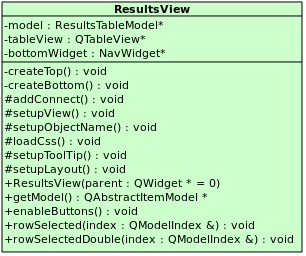
\includegraphics[width=0.45\linewidth]{./Content/Immagini/view/ResultsView.png}
			\caption{Classe ResultsView: attributi e metodi}
			\label{cl_ResV}
\end{figure}
\paragraph{Descrizione \\}
Classe che rappresenta il widget per la visualizzazione di tutte le analisi effettuate contenute dentro a \project{}.Contiene sia le analisi complete, effettuate con successo sia quelle interrotte che quelle incomplete.
\paragraph{Utilizzo\\}
La classe implementerà i metodi virtuali puri della superclasse inoltre darà la possibilità all'utente di visualizzare l'elenco di tutte le analisi effettuate, e di aprire una nuova finestra per vedere nel dettaglio i risultati di una specifica analisi.
\paragraph{Classi ereditate\\}
\begin{itemize}
\item Window::APanel.
\end{itemize}
%%%%%%%ATTRIBUTI%%%%%%%%%%%
\paragraph{\textcolor{black}{Attributi\\}}
%tabelView
\color{teal}\verb!-tableView: QTableView*!
\color{black}
\begin{quote}
Contiene la lista di tutte le analisi effettuate anche se non complete (non eseguite su tutti i \subject del \dataset{}) e interrotte.
\end{quote}
%bottomWidget
\color{teal}\verb! bottomWidget:NavWidget*!
\color{black} 
\begin{quote}
Puntatore al widget che rappresenta la parte bassa della finestra contentente i pulsanti per tornare indietro,e la visualizzazione della guida interattiva.
\end{quote}
%%%%%%%%%  METODI
\paragraph{\textcolor{black}{Metodi\\}}
%costruttore
\color{blue}\verb! + ResultsView(parent : QWidget*=0)!
\begin{quote}
\color{black}Costruttore per la classe ResultsView. \\
\textbf{Argomenti}
\begin{itemize}
\item parent: QWidget*=0  \\ Puntatore al QWidget padre di ResultsView.
\end{itemize}
\end{quote}
%setupLayout()
\color{blue}\verb! #setupLayout():void!
\begin{quote}
\color{black} Metodo che implementa il contratto fornito dalla classe astratta \hyperref[speAPanel]{APanel}.
\begin{itemize}
\item questo metodo deve essere marcato virtuale;
\item questo metodo è stato ridefinito.
\end{itemize}
\end{quote} 
%createTop
\color{blue}\verb! -createTop():void!
\begin{quote}
\color{black} Metodo che ha il compito di costruire la parte in alto del widget contenente l'elenco dei \subject e a lato lo spazio per visualizzare le informazioni.
\end{quote} 
%createButtom
\color{blue}\verb! -createButtom():void!
\begin{quote}
\color{black} Metodo che ha il compito di costruire la parte in basso del widget contenente il pulsante per ritornare alla pagine iniziale, e per l'accesso alla guida.
\end{quote}
%setupTopLayout
\color{blue}\verb! -setupTopLayout():void!
\begin{quote}
\color{black} Metodo che ha il compito di impostare la parte alta del layout della finestra.
\end{quote}  
%LOADCSS
\color{blue}\verb! #loadCss():void!
\begin{quote}
\color{black} Metodo che implementa il contratto fornito dalla classe astratta \hyperref[speAPanel]{APanel}.\\
 \textbf{Note}
 \begin{itemize}
  \item questo metododeve essere marcato virtuale;
 \item questo metodo è stato ridefinito.
 \end{itemize}
\end{quote} 
%setupObjectName
\color{blue}\verb! #setupObjectName():void!
\begin{quote}
\color{black}Metodo che implementa il contratto fornito dalla classe astratta \hyperref[speAPanel]{APanel}.\\
 \textbf{Note}
 \begin{itemize}
  \item questo deve essere marcato virtuale;
 \item questo metodo è stato ridefinito.
 \end{itemize}
\end{quote} 
%setupToolTip
\color{blue}\verb! #setupToolTip():void!
\begin{quote}
\color{black}Metodo che implementa il contratto fornito dalla classe astratta \hyperref[speAPanel]{APanel}.\\
 \textbf{Note}
 \begin{itemize}
 \item questo metodo deve essere marcato virtuale;
 \item questo metodo è stato ridefinito.
 \end{itemize}
\end{quote} 
%addConnect
\color{blue}\verb! #addConnect():void!
\begin{quote}
\color{black}Metodo che implementa il contratto fornito dalla classe astratta \hyperref[speAPanel]{APanel}.\\
 \textbf{Note}
 \begin{itemize}
 \item questo metodo deve essere marcato costante;
 \item questo metodo deve essere marcato virtuale;
 \item questo metodo è stato ridefinito.
 \end{itemize}
\end{quote} 
%setupView
\color{blue}\verb! #setupView():void!
\begin{quote}
\color{black}Metodo che implementa il contratto fornito dalla classe astratta \hyperref[speAPanel]{APanel}.\\
 \textbf{Note}
 \begin{itemize}
 \item questo metodo deve essere marcato virtuale;
 \item questo metodo è stato ridefinito.
 \end{itemize}
\end{quote}


